\documentclass{article}
\usepackage{amsmath} % Voor wiskundige formules
\usepackage[a4paper, margin=2cm]{geometry} % Voor paginamarges
\usepackage[utf8]{inputenc} % Voor het weergeven van speciale karakters
\usepackage[dutch]{babel} % Voor taal-specifieke typografie
%\usepackage{unicode-math} % Voor het gebruik van Unicode-symbolen
\usepackage{graphicx}

\title{Aandrijftechniek Opdrachten}

\author{
  Vollmuller, Michel\\
  1809572\\
  \texttt{michel.vollmuller@student.hu.nl}
}

\begin{document}
\maketitle

\begin{abstract}
    Dit document bevat de opdrachten 1 t/m 4 voor de cursus Aandrijftechniek tijdens semester 6 van de opleiding Eleketrotechniek bij de Hogeschool Utrecht. De opdrachten betreffen verschillende soorten motoren die allemaal behandeld worden tijdens de cursus. Bij de oprachten zijn vraag en antwoord gedefinieerd.
\end{abstract}

\tableofcontents

\newpage

\section{Opdracht 1 Gelijkstroommotoren}
\begin{center}
    \textbf{Motor Specifications}
\end{center} 

\begin{align*}
    &\text{Nominal Voltage (U\textsubscript{klem\_nom)}:} & 24 \, \text{V} \\
    &\text{Nominal Current (I\textsubscript{klem\_nom)}:} & 10.71 \, \text{A} \\
    &\text{Efficiency:} & 70\% \\
    &\text{No-load Speed (n\textsubscript{no\_load}):} & 1910 \, \text{rpm} \quad (T\textsubscript{nullast} = 0 \, \text{Nm}) \\
    &\text{Nominal Shaft Torque (T\textsubscript{as\_nom}):} & 1.0 \, \text{Nm}
\end{align*}


\begin{enumerate}
    \item [a.] \textbf{Bepaal het nominale vermogen op de as van de motor ($P_{\text{as\_nom}}$):}
    
        $P_{\text{nominaal}} = \text{Nominal Voltage} \times \text{Nominal Current} \times \text{Efficiency} = 24 \times 10,71 \times 0.70 = 179,93W$



    \item [b.] \textbf{Teken de koppeltoeren-karakteristiek van de motor. Geef duidelijk aan bij
    welke waarde de karakteristiek de verticale as snijdt en bij welke waarde de
    karakteristiek de horizontale as snijdt.}

        % $T\textsubscript{stall} = \frac{U\textsubscript{klem}}{R\textsubscript{r}} \times K\textsubscript{em} = \frac{U\textsubscript{klem}}{\frac{U\textsubscript{klem}}{I\textsubscript{klem}}} \times K\textsubscript{em} = \frac{24}{\frac{24}{10,71}} \times 0,09 = 0,96 \text{ Nm}$

        $T\textsubscript{stall} = 1 \text{ Nm}$

        $\omega_{null} = \frac{P_{as_nominaal}}{T_{as}} = \frac{179,93}{1} = 179,93 \text{ rad/s}$

        \begin{figure}[h]
            \centering
            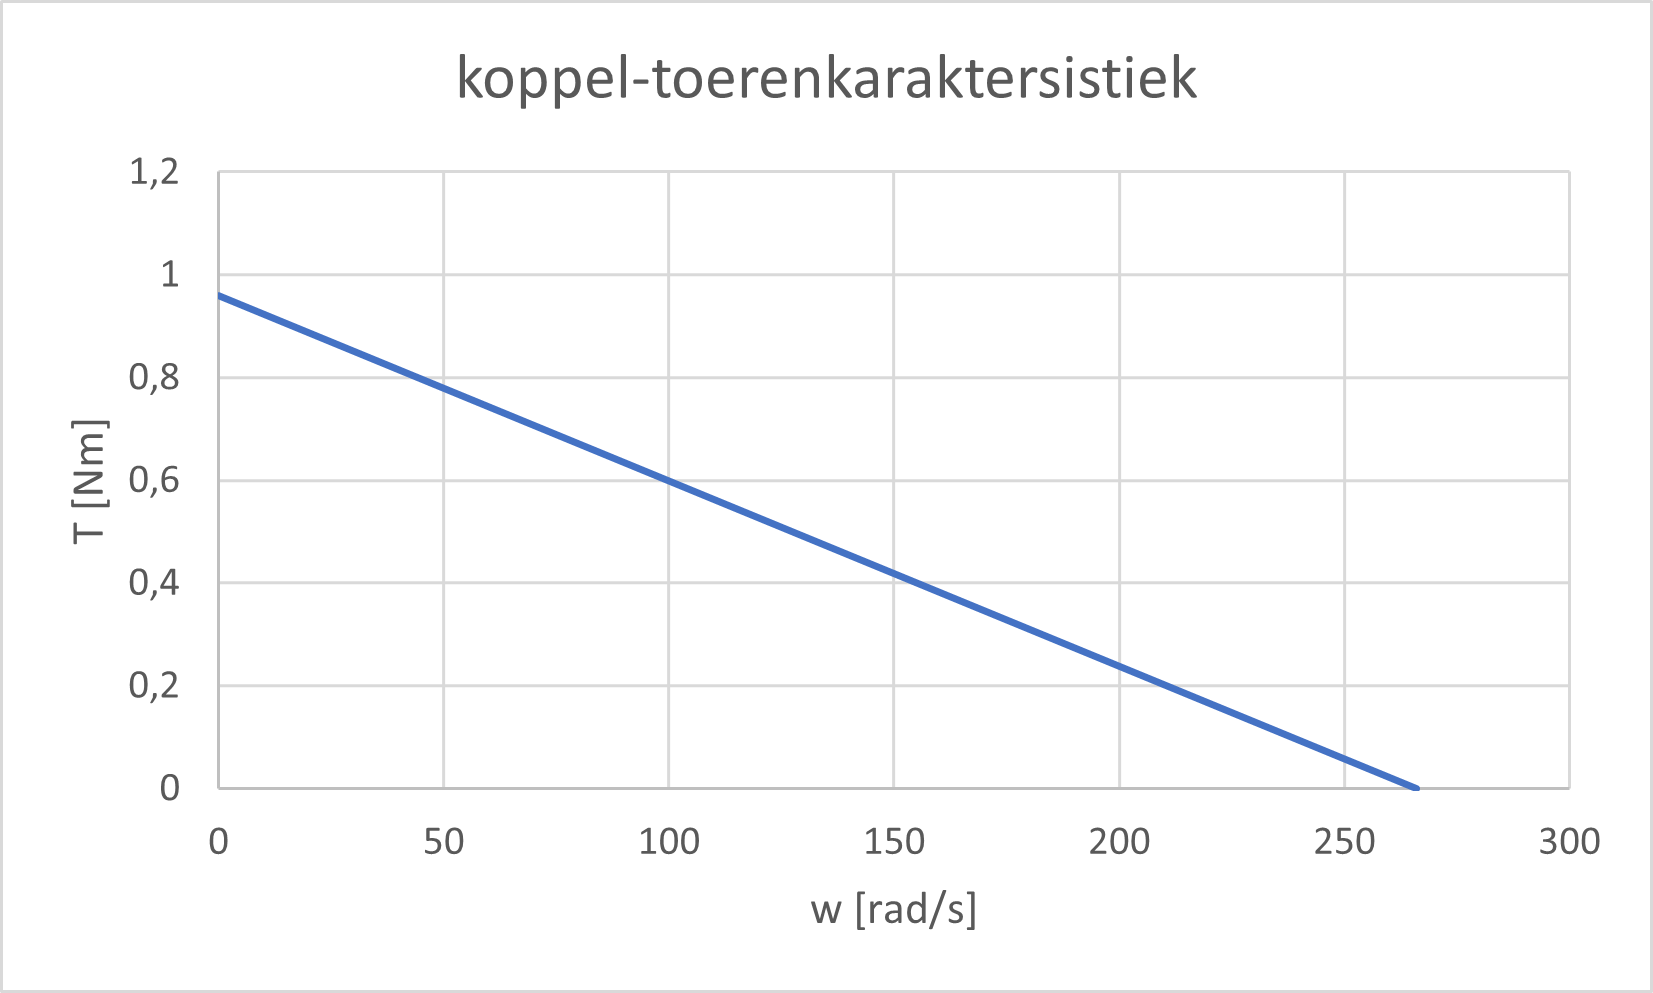
\includegraphics[scale=0.7]{koppel-toerenkarakteristiek 1b.png}
            \caption{koppel-toerenkarakteristiek}
        \end{figure}

    \item [c.] \textbf{Een belangrijke parameter van de motor is de motorconstante $K_{\text{em}}$.
    Bereken deze.}

        $K\textsubscript{em} = \frac{U\textsubscript{klem}}{\omega\textsubscript{nullast}} = \frac{24}{200} = 0.12 \text{ V/ rad/s}$

\item [d.] \textbf{De motor wordt gebruikt voor het aandrijven van een toerental onafhankelijke
    last van $T_{\text{last}}$ = 200 mNm. De klemspanning van de motor is ingesteld op 24V
    Bepaal nu het werkpunt van de motor: het toerental en het koppel. Wat is bij dit werkpunt de opgenomen stroom?}     

        $\text{toerental} -> 0,2=-0,05x + 9,9998 -> x = 196 rad/s = 1871,66 rpm $
    
        $\text{koppel} = 0,2 Nm$
        
        $\text{stroom} = \frac{koppel}{motorconstante} = \frac{0,2}{0,12} = 1,67 A$

    \item [e.] \textbf{De motor wordt gebruikt voor het aandrijven van een toerental onafhankelijke
    last van $T_{\text{last}}$ = 200 mNm. Dus dat is nog dezelfde situatie als bij opgave d).
    De klemspanning wordt nu echter 12V.
    Bepaal nu weer het werkpunt van de motor: het toerental en het koppel.
    Wat is bij dit werkpunt de opgenomen stroom?}

    Er van uit gaande dat als de spanning halveerd dat het toerental dan ook halveerd =

    $\text{toerental} \Rightarrow 0,2=-0,05x + 9,9998 \Rightarrow x = 96 rad/s = 916,73 rpm  $

    $\text{koppel} = 0,2 Nm$
    
    $\text{stroom} 
    = \frac{koppel}{motorconstante} 
    = \frac{koppel}{\frac{U\textsubscript{klem}}{\omega\textsubscript{nullast}}}
    = \frac{0,2}{\frac{12}{100}} = 1,67 A$

\end{enumerate}


\newpage
\section{Opdracht 2 Asynchromemotoren}
\textbf{Onderbouw je antwoorden altijd door beredenering en/of berekening.}

Een driefasen asynchrone motor is aangesloten op een spanning van 400V/50Hz.
De motor drijft een last aan waarvan het koppel recht evenredig is met het toerental.
Bij het nominale toerental bedraagt het lastkoppel 100 Nm.
Voor de combinatie motor en last is het nominale toerental 1440 rpm.
Voor de motor geldt verder dat het aanloopkoppel 0,7 maal het nominale koppel is
$(T_{aanloop} = 0,7 \times T_{nom})$ en dat het kipkoppel gelijk is aan $T_{kip} = 2 \times T_{nom}$.

\begin{enumerate}
    \item [a.] \textbf{Wat is het aantal poolparen van deze motor? Bepaal de slip van de motor bij nominaal bedrijf.}
    
        Poolparen:
        $ P = \frac{60 \times f}{n_{s}} = \frac{60 \times 50}{\approx1440} \approx 2 poolparen $

        Slip:
        $slip 
        = \frac{n_{s} - n_{r}}{n_{s}} 
        = \frac{\frac{Hz*60}{P} - n_{r}}{\frac{Hz*60}{P}}
        = \frac{1500 - 1440}{1500} \times 100 
        = 4\% slip$

    \item [b.] \textbf{Bereken het nominale asvermogen.}

    $P_{nominale} 
    = \frac{T_{nominale} \times 2\pi \times n_{nominale}}{60}= \frac{100 \times 2\pi \times 1440}{60} 
    = 15079,65 Watt \approx 15 kW$


    \item [c.] \textbf{Teken in één grafiek: De koppeltoerenkarakteristiek van de motor en de koppeltoerenkarakteristiek van de last. Geef duidelijk de kenmerkende waarden aan en laat zien hoe je aan die waarden komt.}

        \begin{figure}[h]
            \centering
            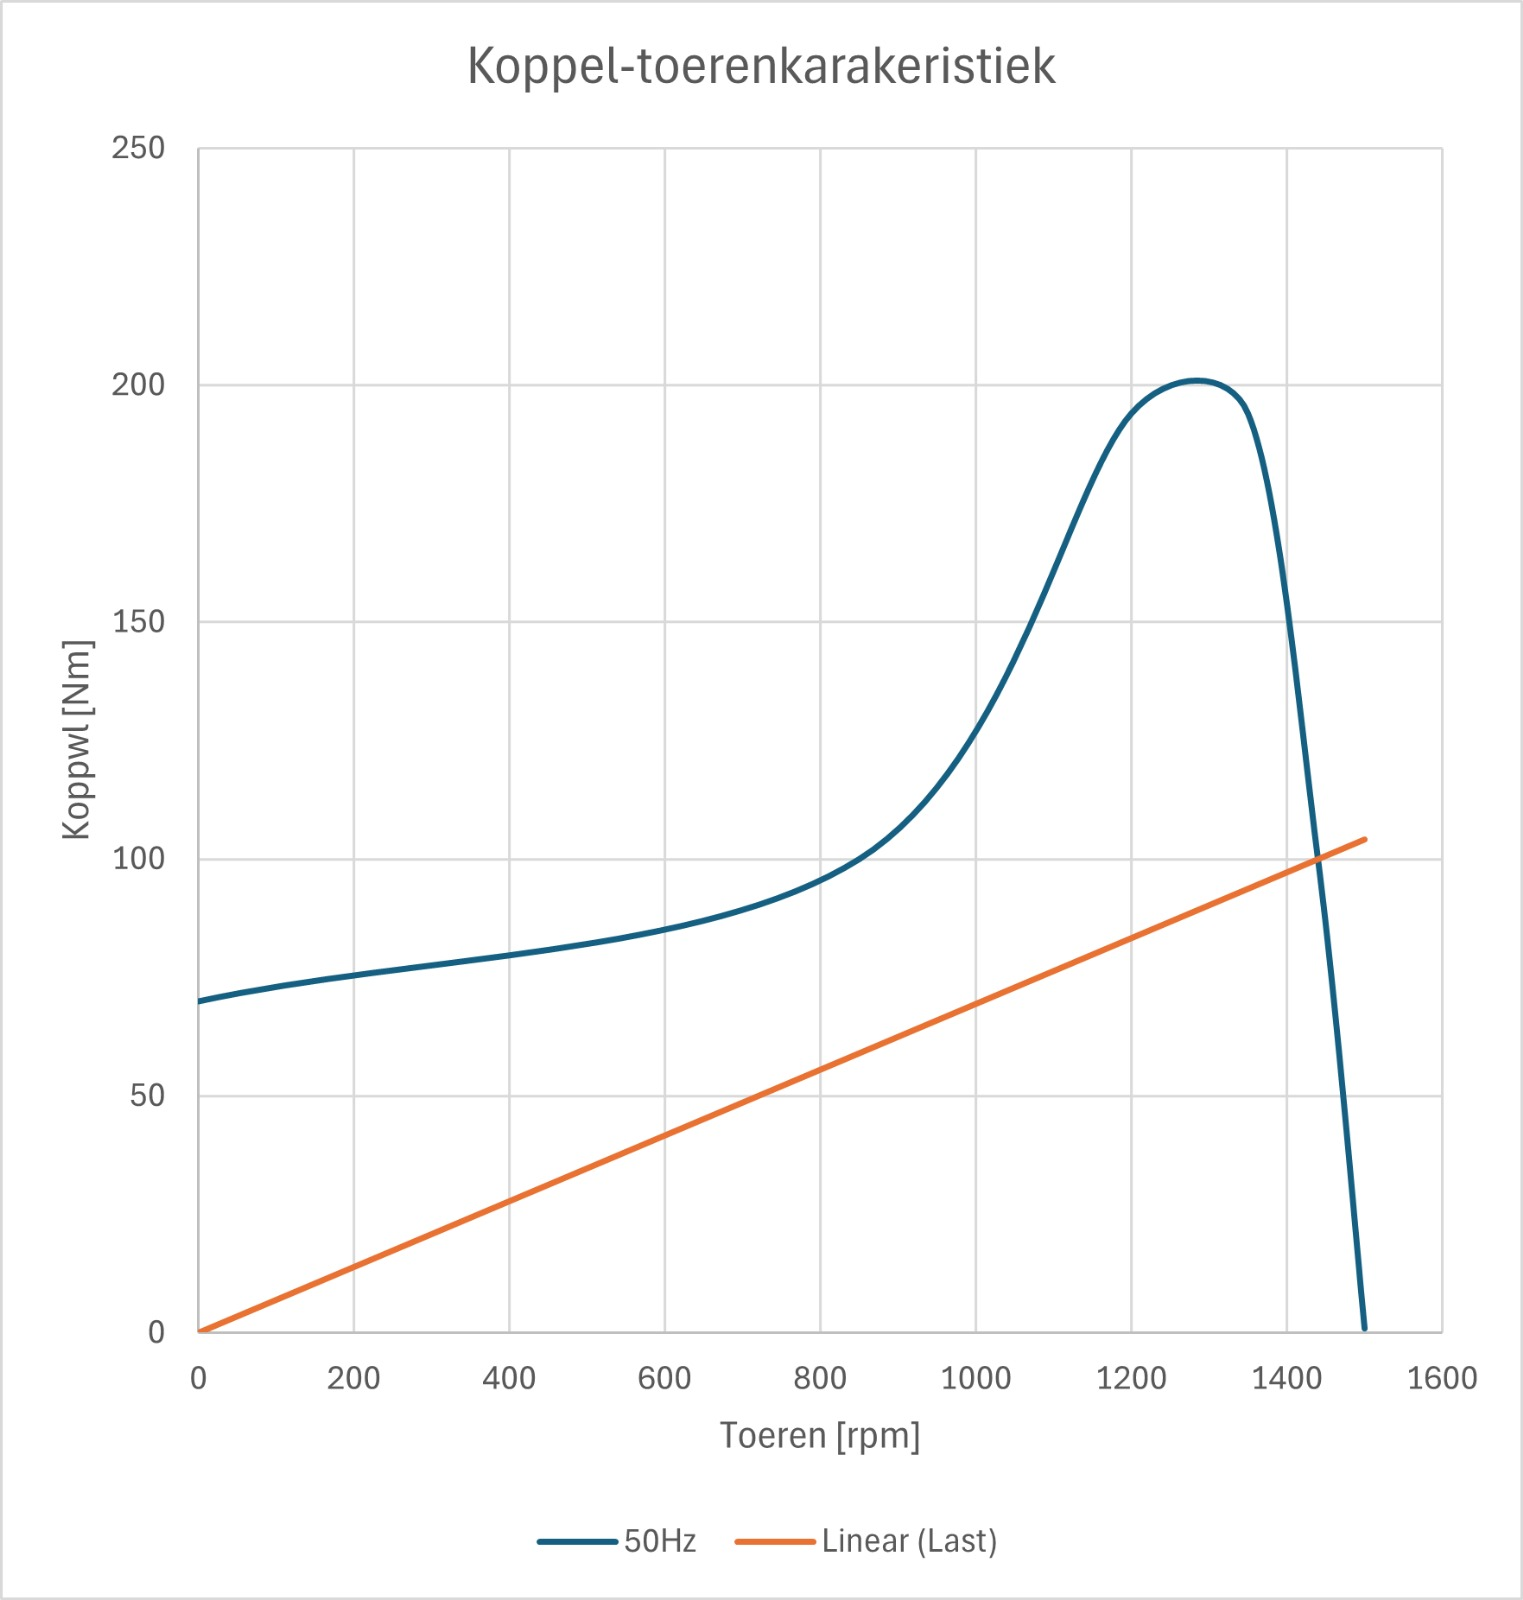
\includegraphics[scale=0.11]{kopppel-toerenkarakteristiek.jpg}
            \caption{koppel-toerenkarakteristiek}
        \end{figure}

    \item [d.] \textbf{Met behulp van een frequentieregelaar wordt het toerental gehalveerd $(n = 720 rpm)$. Wat moet de spanning en frequentie van de frequentieregelaar zijn om dit toerental in te kunnen stellen? Licht je antwoord kort toe.} 
        
        \[ frequentie 
        = \frac{n \times P}{60} 
        = \frac{720 \times 2}{60} 
        = 24 Hz \]
        
        Wat betreft de spanning, wordt deze meestal gehandhaafd op de nominale spanning van de motor, in dit geval \( 400 \, \text{V} \). De frequentieregelaar past de frequentie aan om het gewenste toerental te bereiken terwijl de spanning op het nominale niveau blijft om een goede werking van de motor te garanderen.
    

    \item [e.] \textbf{Wat verandert er aan de motorkarakteristiek als de frequentie van de frequentieregelaar $100 Hz$ is en de spanning gelijk blijft?
    Schets de nieuwe motorkarakteristiek en licht je antwoord kort toe.}

        \begin{figure}[h]
            \centering
            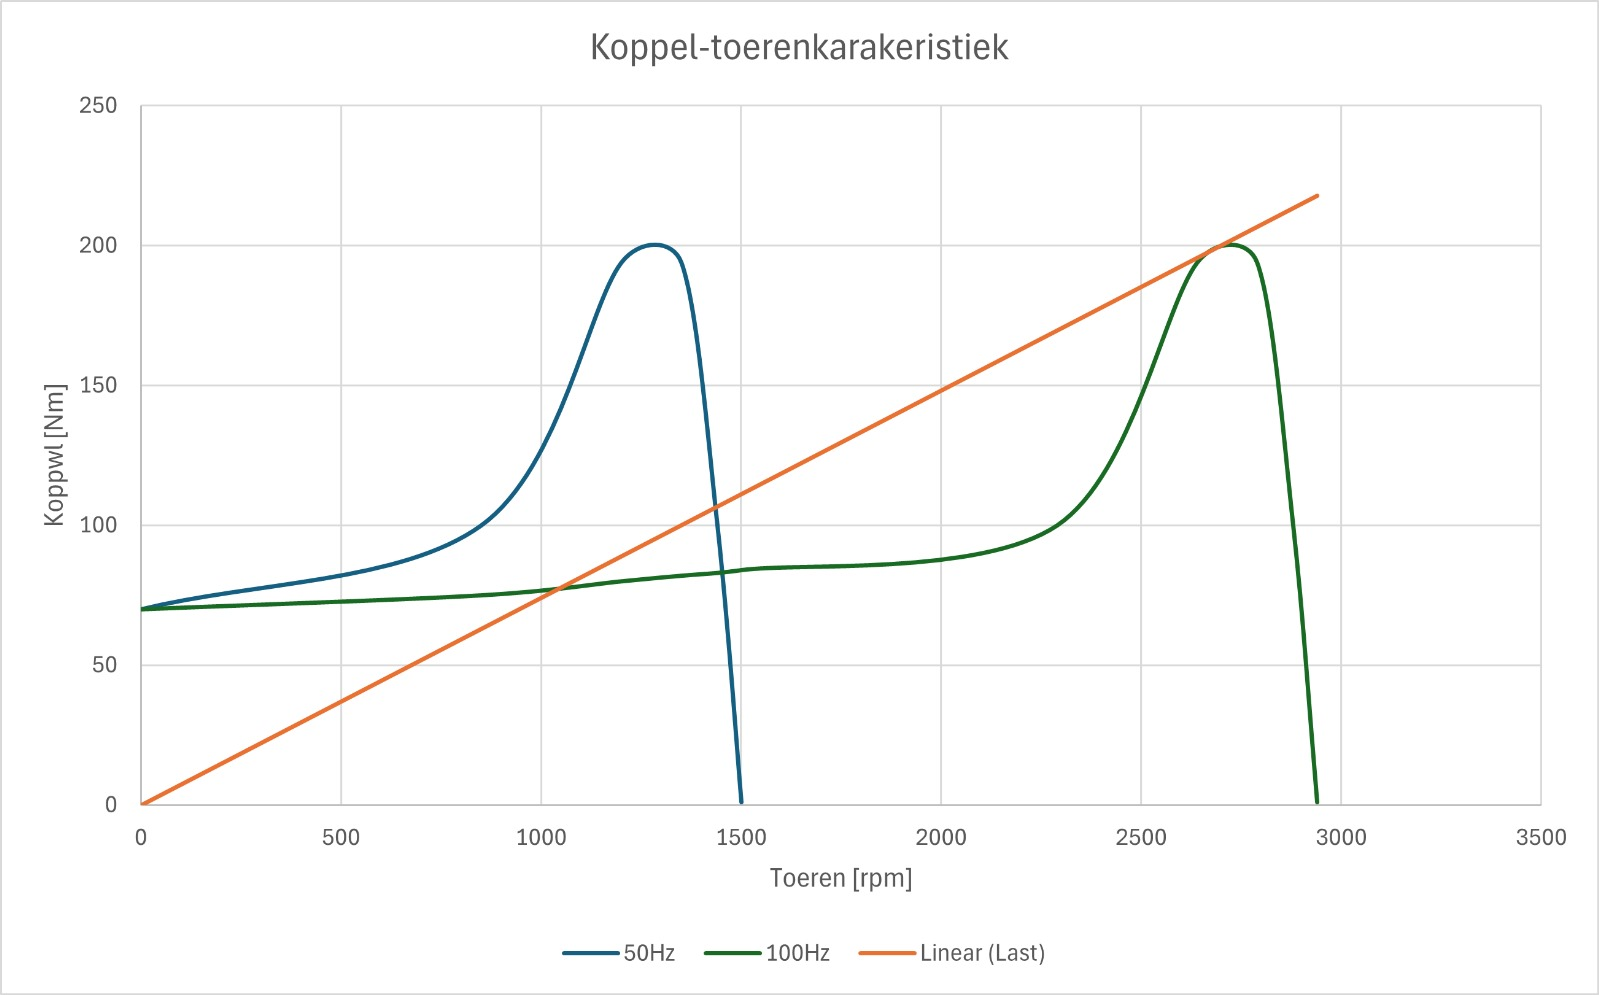
\includegraphics[scale=0.13]{2e.jpg}
            \caption{koppel-toerenkarakteristiek}
        \end{figure}

\end{enumerate}

\newpage
\section{Opdracht 3 Synchromemotoren}
\textbf{Onderbouw je antwoorden altijd door beredenering en/of berekening.}

Gegeven is een synchrone driefasen motor met een permanent magneet rotor die wordt aangestuurd met een frequentieregelaar. Het aandrijfsysteem (motor en regelaar) is ontworpen op een nominale spanning van 400V/100Hz. Bij een instelling van de frequentieregelaar op 60 Hz heeft de motor de onderstaande
koppel-toerenkarakteristiek.

\begin{figure}[h]
    \centering
    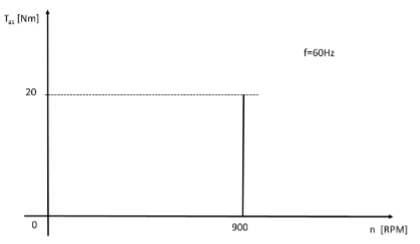
\includegraphics[scale=1.5]{3-uitleg.png}
\end{figure}

\begin{enumerate}
    \item [a.] \textbf{Bepaal de polen van deze motor}
    
        Poolparen:
        $ P = \frac{60 \times f}{n_{s}} = \frac{60 \times 60}{900} = 4 poolparen $

    \item [b.] \textbf{Bepaal de lasthoek van de motor bij een lastkoppel van 10 Nm.}
    
        $ \delta = 90 \times \frac{T_{last}}{T_{max}} = 90 \times \frac{10}{20} = 45 graden$

\end{enumerate}

De motor wordt gebruikt om een last aan te drijven waarvan de koppel-toerenkarakteristiek tijdens bedrijf kan variëren in het rode gebied dat is aangegeven in onderstaand figuur.
\begin{figure}[h]
    \centering
    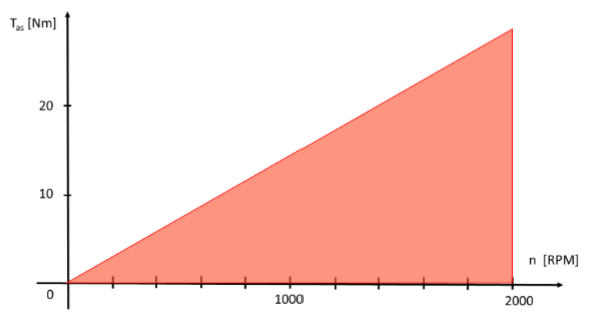
\includegraphics[scale=1]{3b-uitleg.png}
\end{figure}

\begin{enumerate}
    \item [c.] \textbf{Wat is het maximale koppel en toerental van het aandrijfsysteem (motor en regelaar) zodat voldaan wordt aan de eis dat het toerental constant blijft?}
    
        $rpm_{max} = \frac{f \times 60}{p} = \frac{100 \times 60}{4} = 1500rpm$

        Omdat je koppel toerenkarakteristiek over de horizontale as verschuift omdat je rpm meer wordt blijft je koppel gelijk. ofterwijl 20Nm.


    \item [d.] \textbf{Bepaal het maximale vermogen dat de motor op de last kan overbrengen bij een lastkoppel van 10 Nm.}     
    
        $ P_{uit} = \omega_{s} \times T_{em} = 157 \times 10 = 1570 Watt $

        $ \omega_{s} 
        = \frac{2 \times \pi \times rpm}{60} 
        = \frac{2 \times \pi \times 1500}{60} 
        = 157 rad/s$

    \item [e.] \textbf{Wat is het maximale toerental van de motor waarmee een constante last van 20 Nm aangedreven kan worden?}
    
        1500rpm is het macimale toerental van de motor waarmee een last van 20Nm aangedreven kan worden.\\
        Zie ook opgave c en d.

\end{enumerate}

\newpage
\section{Opdracht 4 stappenmotoren}
\textbf{Onderbouw je antwoorden altijd door beredenering en/of berekening.}

Voor een tweefasen PM-stappenmotor is het koppel voor fase A en B:
\begin{align*}
    T_{em,A} &= 6 \cdot i_{s,A} \cdot \sin(4\theta) \, \text{mNm} \\
    T_{em,B} &= 6 \cdot i_{s,B} \cdot \sin(4\theta - 90^\circ) \, \text{mNm}
    \end{align*}\\
Voor volstapbedrijf geldt: \(i_{s,A} = i_{s,B} = 0.5 \, \text{A}\).\\
Men wil met behulp van ministappen extra stappen creeren.    


\begin{enumerate}
    \item [a.] \textbf{Hoeveel ministappen heb je nodig om nullaststenden van $0^\circ ; 2,25^\circ ; 4,5^\circ ; 6,75^\circ ; 9^\circ ; 11,25^\circ$ etc te krijgen?}
    
        Hier komen antwoorden

    \item [b.] \textbf{Bepaal de lasthoek van de motor bij een lastkoppel van 10 Nm.}
    
        Hier komen antwoorden

    \item [c.] \textbf{Waarom zal een ministap altijd naar de positie van de nullaststand willen
    gaan?}
    
        Hier komen antwoorden


    \item [d.] \textbf{Kan deze stappenmotor een lastkoppel van 5 mNm verplaatsen?
    Licht je antwoord kort toe.}     
    
        Hier komen antwoorden

    \item [e.] \textbf{Als je bij b) geen antwoord hebt gevonden, ga dan uit van 10 ministappen.
    Hoe groot zijn de stromen $i_{s,A}$ en $i_{s,B}$ om elke afzonderlijke ministap te kunnen
    maken?}
    
        hier komen antwoorden

\end{enumerate}


\end{document}
